\renewcommand{\NomeBloco}{Multiplexador 7x1}
\renewcommand{\NomePTab}{tab_\NomeBloco}
\renewcommand{\NomeSTab}{tab_\NomeBloco2}
\renewcommand{\NomePFig}{fig_\NomeBloco}
\renewcommand{\NomeSFig}{fig_\NomeBloco2}
\renewcommand{\NomeTTab}{tab_\NomeBloco3}

\section{\NomeBloco}

O bloco \NomeBloco{} tem a fun{\c c}\~ao de colocar na sa\'ida o valor correspondente \'a entrada selecionada. Nesse bloco, 7 entradas distintas podem ser selecionadas. A \autoref{\NomePTab} indica a Tabela Verdade do bloco. Embora tenha uma l\'ogica digital, o circuito permite entradas e sa\'idas anal\'ogicas.

\begin{table}[htbp]

\caption{Tabela Verdade do bloco \NomeBloco}%
\label{\NomePTab}
\centering
\begin{tabular}{ccccc}
    \toprule
    D0 & D1 & D2 & D3 & Out \\
    \midrule \midrule
    0 & 0 & 0 & 0 & In0 \\
    \midrule
    0 & 1 & 0 & 0 & In1 \\
    \midrule
    1 & 0 & 0 & 0 & In2 \\
    \midrule
    1 & 1 & 0 & 0 & In3 \\
    \midrule
    X & X & 0 & 1 & In4 \\
    \midrule
    X & X & 1 & 0 & In5 \\
    \midrule
    X & X & 1 & 1 & In6 \\
\bottomrule

\end{tabular}
\fonte{Produzido pelo autor.}
\end{table}

O bloco apresenta as defini{\c c}\~oes de sinais de entrada e sa\'ida referidos na \autoref{\NomeSTab}.

\begin{table}[htbp]
\caption{Sinais do bloco \NomeBloco}
\label{\NomeSTab}
\centering
\begin{tabular}{ccl}

    \toprule
    Sinal & Tipo    & Descri{\c c}\~ao        \\
    \midrule \midrule
    D0    & Entrada & Primeira entrada de sele{\c c}\~ao de sa\'ida \\
    \midrule
    D1    & Entrada & Segunda entrada de sele{\c c}\~ao de sa\'ida \\
    \midrule
    D2    & Entrada & Segunda entrada de sele{\c c}\~ao de sa\'ida \\
    \midrule
    D3    & Entrada & Segunda entrada de sele{\c c}\~ao de sa\'ida \\
    \midrule
    Vout & Sa\'ida & Sa\'ida do Multiplexador\\
    \midrule
    \bottomrule
\end{tabular}
\legend{Fonte: Produzido pelo autor}
\end{table}

O circuito projetado para o bloco \'e demonstrado na \autoref{\NomePFig}.

\begin{figure}[htbp]
 \label{NomePFig}
 \centering
    \centering
    \caption{Circuito CMOS projetado para o bloco \NomeBloco} \label{\NomePFig}
    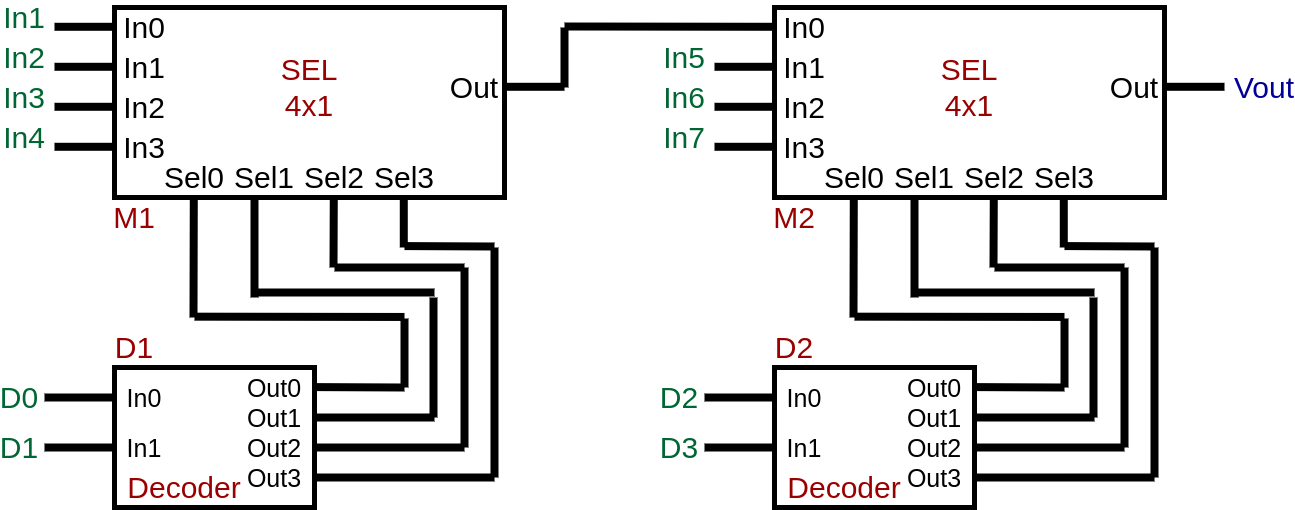
\includegraphics[scale=0.3]{Circuitos/mux7x1.png}
    \legend{Fonte: Produzido pelo autor}
\end{figure}

\begin{figure}[htbp]
 \label{NomeSFig}
 \centering
    \centering
    \caption{Representa{\c c}\~ao em bloco do \NomeBloco} \label{NomeSFig}
    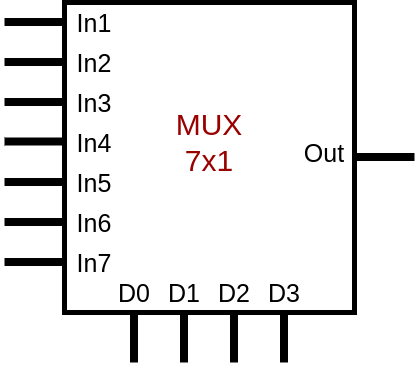
\includegraphics[scale=0.5]{Circuitos/mux7x1_block.png}
    \legend{Fonte: Produzido pelo autor}
\end{figure}
\clearpage